\documentclass{article}
\usepackage[spanish]{babel}
\usepackage[utf8]{inputenc}	
\usepackage{graphicx}
\usepackage{mathtools}
\usepackage{vmargin}
\usepackage{pgfplots}
\usepackage{fancyhdr}

\pgfplotsset{compat=newest}
\setpapersize{A4}
\newcommand*\rfrac[2]{{}^{#1}\!/_{#2}}		

\title{Matemática Superior\\Trabajo Práctico 1}

\author{ Busso, Francisco\\francisco.busso@outlook.com 
    \and Ferraro Trivelli, Giovani\\gftrivelli@frsf.utn.edu.ar
    \and Storani, Miguel\\ miguelignaciostorani@gmail.com
}

\pagestyle{fancy}

\renewcommand{\maketitle}{
    \begin{center}
        
        {\scshape{Universidad Tecnológica Nacional\\Facultad Regional Santa Fe}}
        \vspace{10pt}
        \hrule
        \vspace{10pt}
       

        {\LARGE\bfseries{Matemática Superior\\}}
        \vspace{5pt}
        {\Huge\bfseries{Trabajo Práctico 1B}}

        \vspace{8pt}
        \hrule
        \vspace{8pt}

        Busso, Francisco\\
        \textit{francisco.busso@outlook.com}\\
        \vspace{7pt}
        Ferraro Trivelli, Giovani\\
        \textit{gftrivelli@frsf.utn.edu.ar}\\
        \vspace{7pt}
        Storani, Miguel\\
        \textit{miguelignaciostorani@gmail.com}\\

        % Setea el estilo de la pagina a vacío
        \thispagestyle{empty}
        
        % Terimna la pagina actual
        \newpage
    \end{center}
}

\rhead{Matemática Superior}
\lhead{
\includegraphics[width=3.2cm]{./Imagenes/logo.png}}

\begin{document}
\maketitle
\newpage

\renewcommand{\contentsname}{Índice}
\tableofcontents
\newpage

	\section{Transformada Discreta}
		\subsection{Consideraciones previas}
			\paragraph{}
			Se consideró que la consigna de trasladar los segmentos al origen temporal colocaba a los segmentos en el origen de coordenadas. En la retroalimentación de
			la entrega se nos informó del error y se construyeron nuevamente las matrices de espectro, con los segmenos colocados de manera solicitada. Dado que los resultados
			obtenidos con estas nuevas matrices fueron significativamente similares a los resultados anteriores, el informe se desarrolla con las matrices construidas en primera
			instancia.


		\subsection{Visualización de la matriz}
	        \paragraph{}
	        Una vez separada la función en segmentos y calculadas las Transformadas de Fourier en Tiempo Discreto de cada uno, 
	        se construyó la Matriz de Espectro E utilizando la formula propuesta. Posteriormente se determinaron los valores máximo y mínimo de dicha matriz 
	        y se construyó una nueva matriz de igual dimensión a la matriz de espectro, en la cuál se le asignó a cada posición de la misma un valor entre 0 y 255, 
	        mediante la siguiente fórmula:
	
	        \begin{equation}
	            V_{(i, j)}=\frac{E_{(i, j)}-m}{M-m}*255
	        \end{equation}
	
	        Donde \textit{M} representa al valor máximo de la Matriz de Espectro y \textit{m} al valor mínimo de la misma.
	        Esto se realizó para diferenciar gráficamente las frecuencias predominantes (zonas  brillantes) 
	        de las frecuencias que aportan menos energía (zonas oscuras) a la señal final.
	
	        \begin{figure}[h!]
	            \centering
	            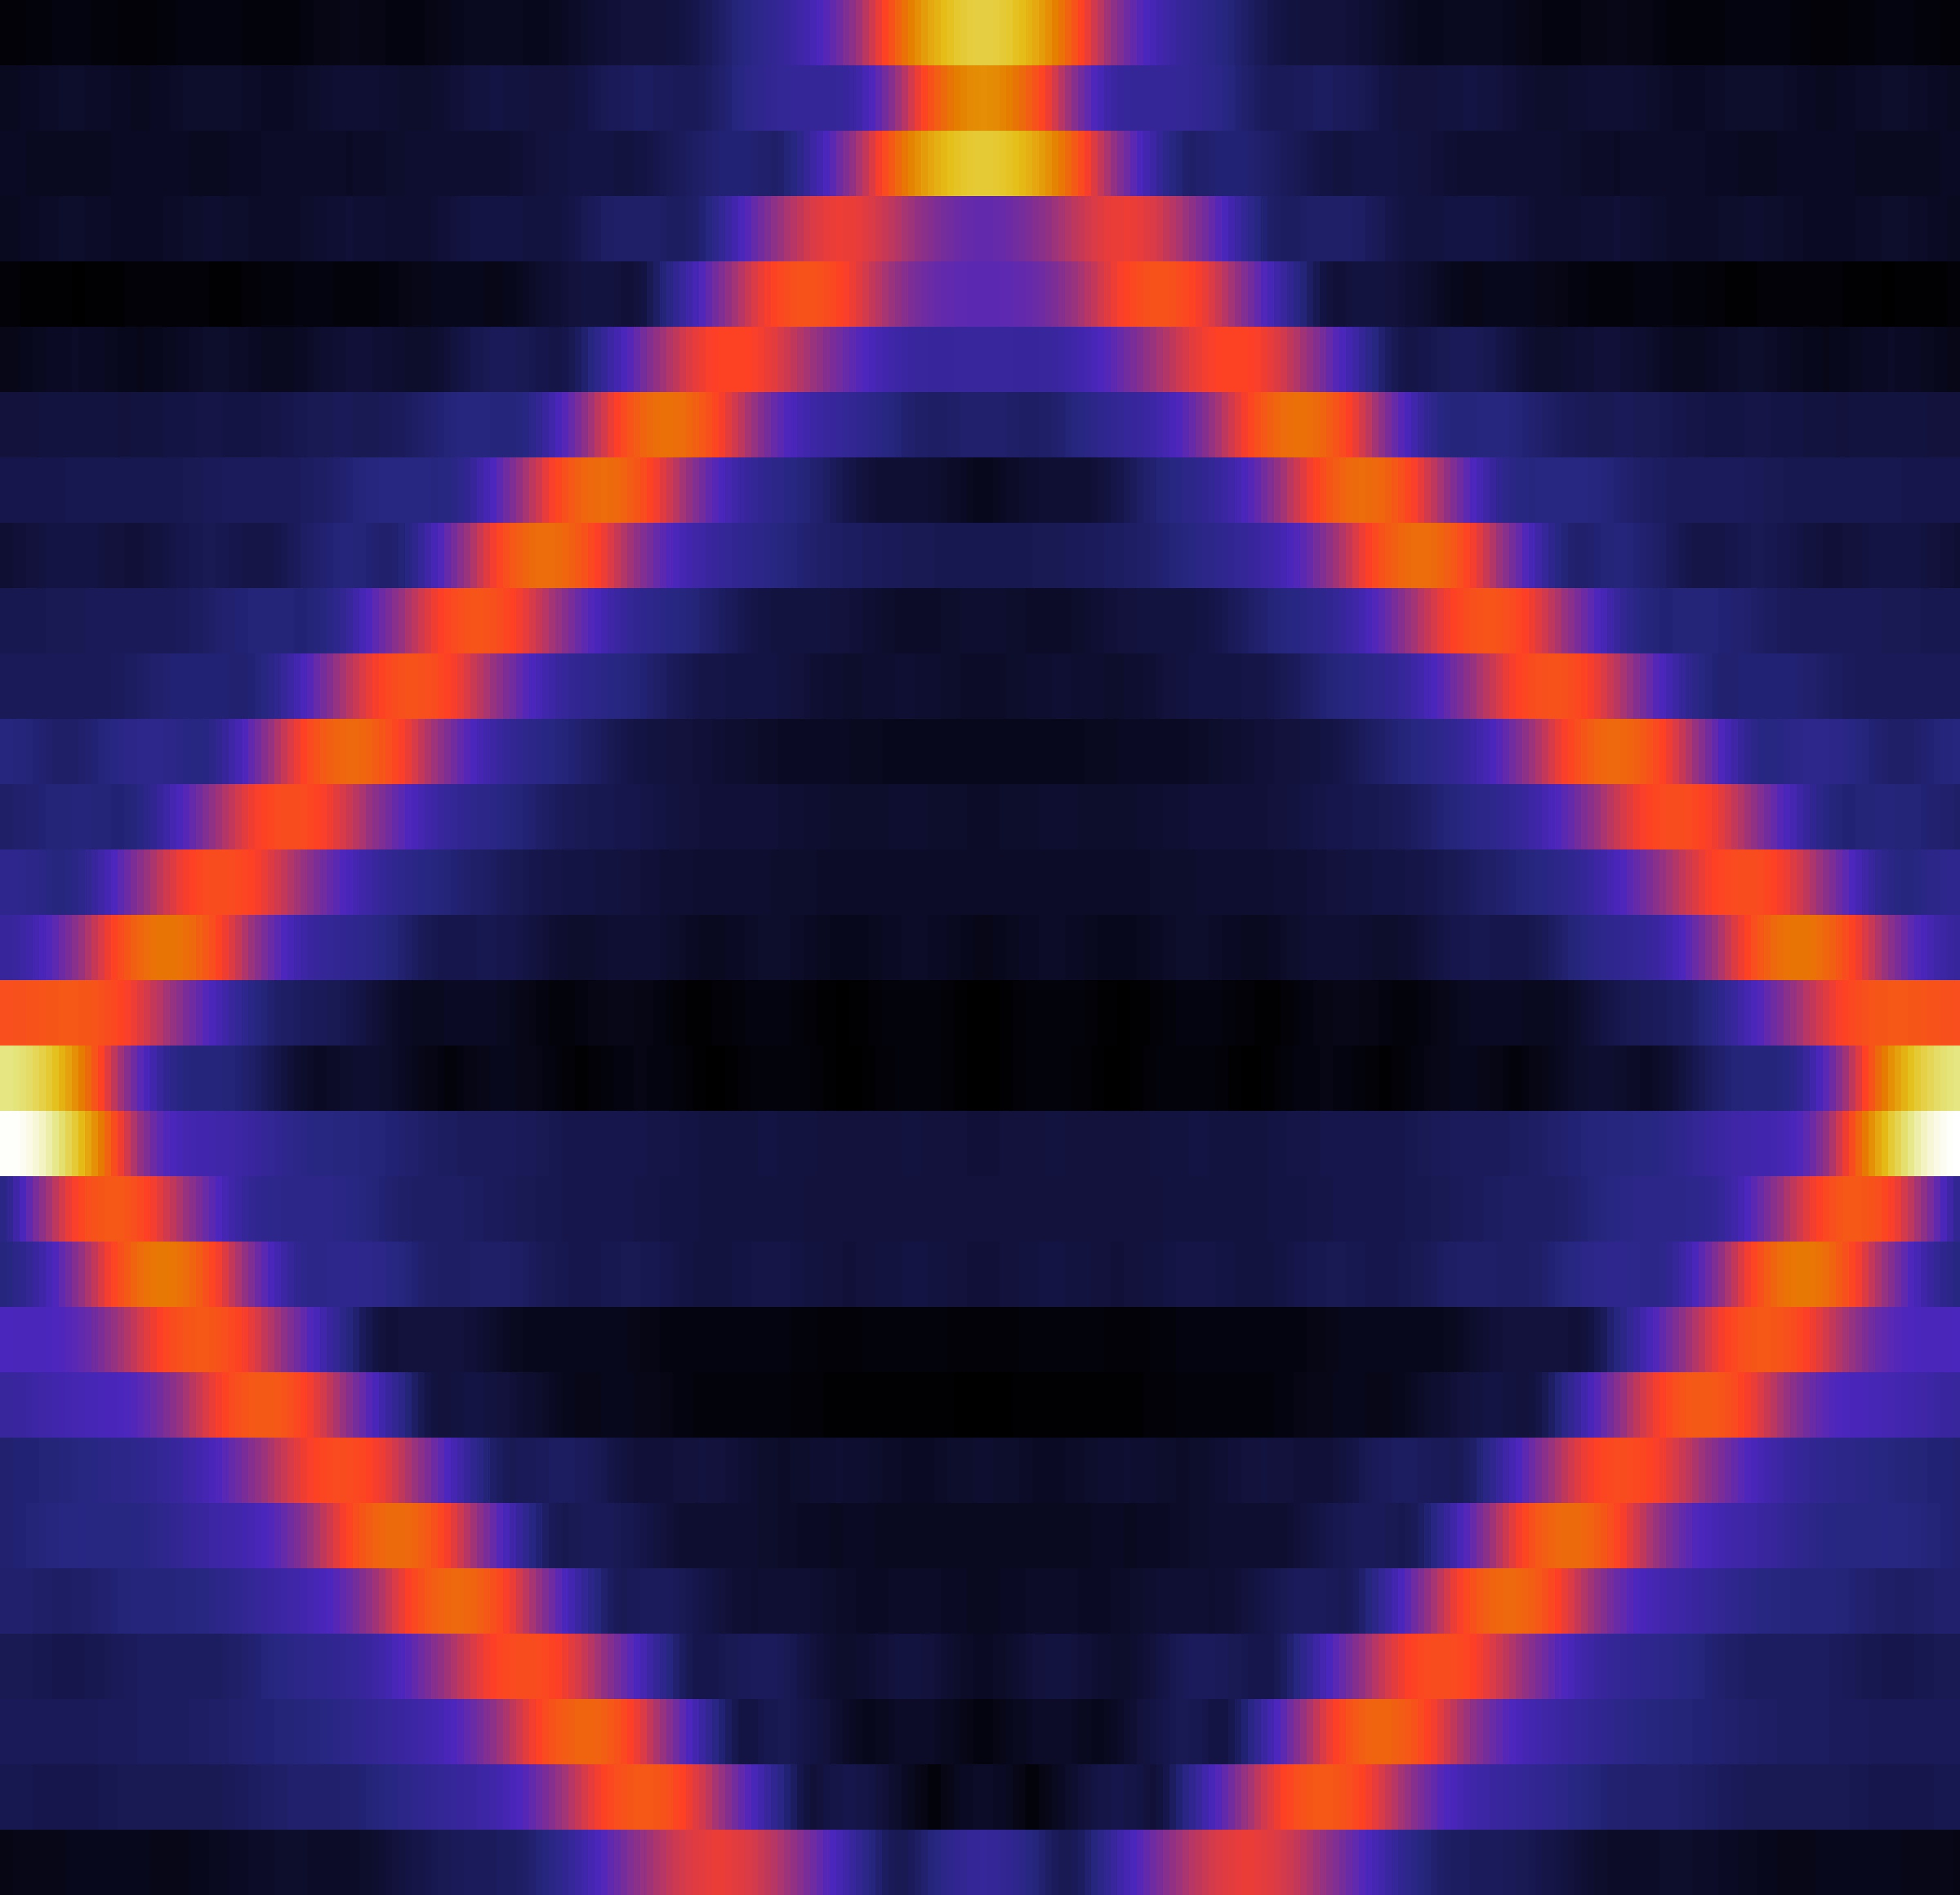
\includegraphics[width=0.5\textwidth]{./Imagenes/Espectrogramas/estudiada.jpg}
	            \caption{Representación gráfica de la Matriz de Espectro}
	            \label{estudiada}
	        \end{figure}
	
	        \paragraph{}

	        \paragraph{}
	        Este procesamiento de los datos fue realizado con el fin de poder analizar más intuitivamente la información presentada en la matriz de espectro generada, 
	        pudiendo así contrastar los diferentes escenarios conocidos contra la señal en estudio e identificar a cuál se asemeja.
	        
	\subsection{Análisis de los resultados}
	        
	        Para analizar la señal propuesta, nos ayudamos de señales conocidas. Para esto se generaron las matrices de espectro para una función de frecuencia constante (figura \ref{constante}) y otra con frecuencia linealmente variable (figura \ref{variable}).
	        A partir de la comparación de la matriz de espectro de la señal en estudio y la matriz de una señal con frecuencia linealmente variable podemos decir que la señal estudiada tiene un comportamiento similar (pero no igual) a una señal con frecuencia variable.
	        
	
	        \begin{figure}[h!]
	            \centering
	            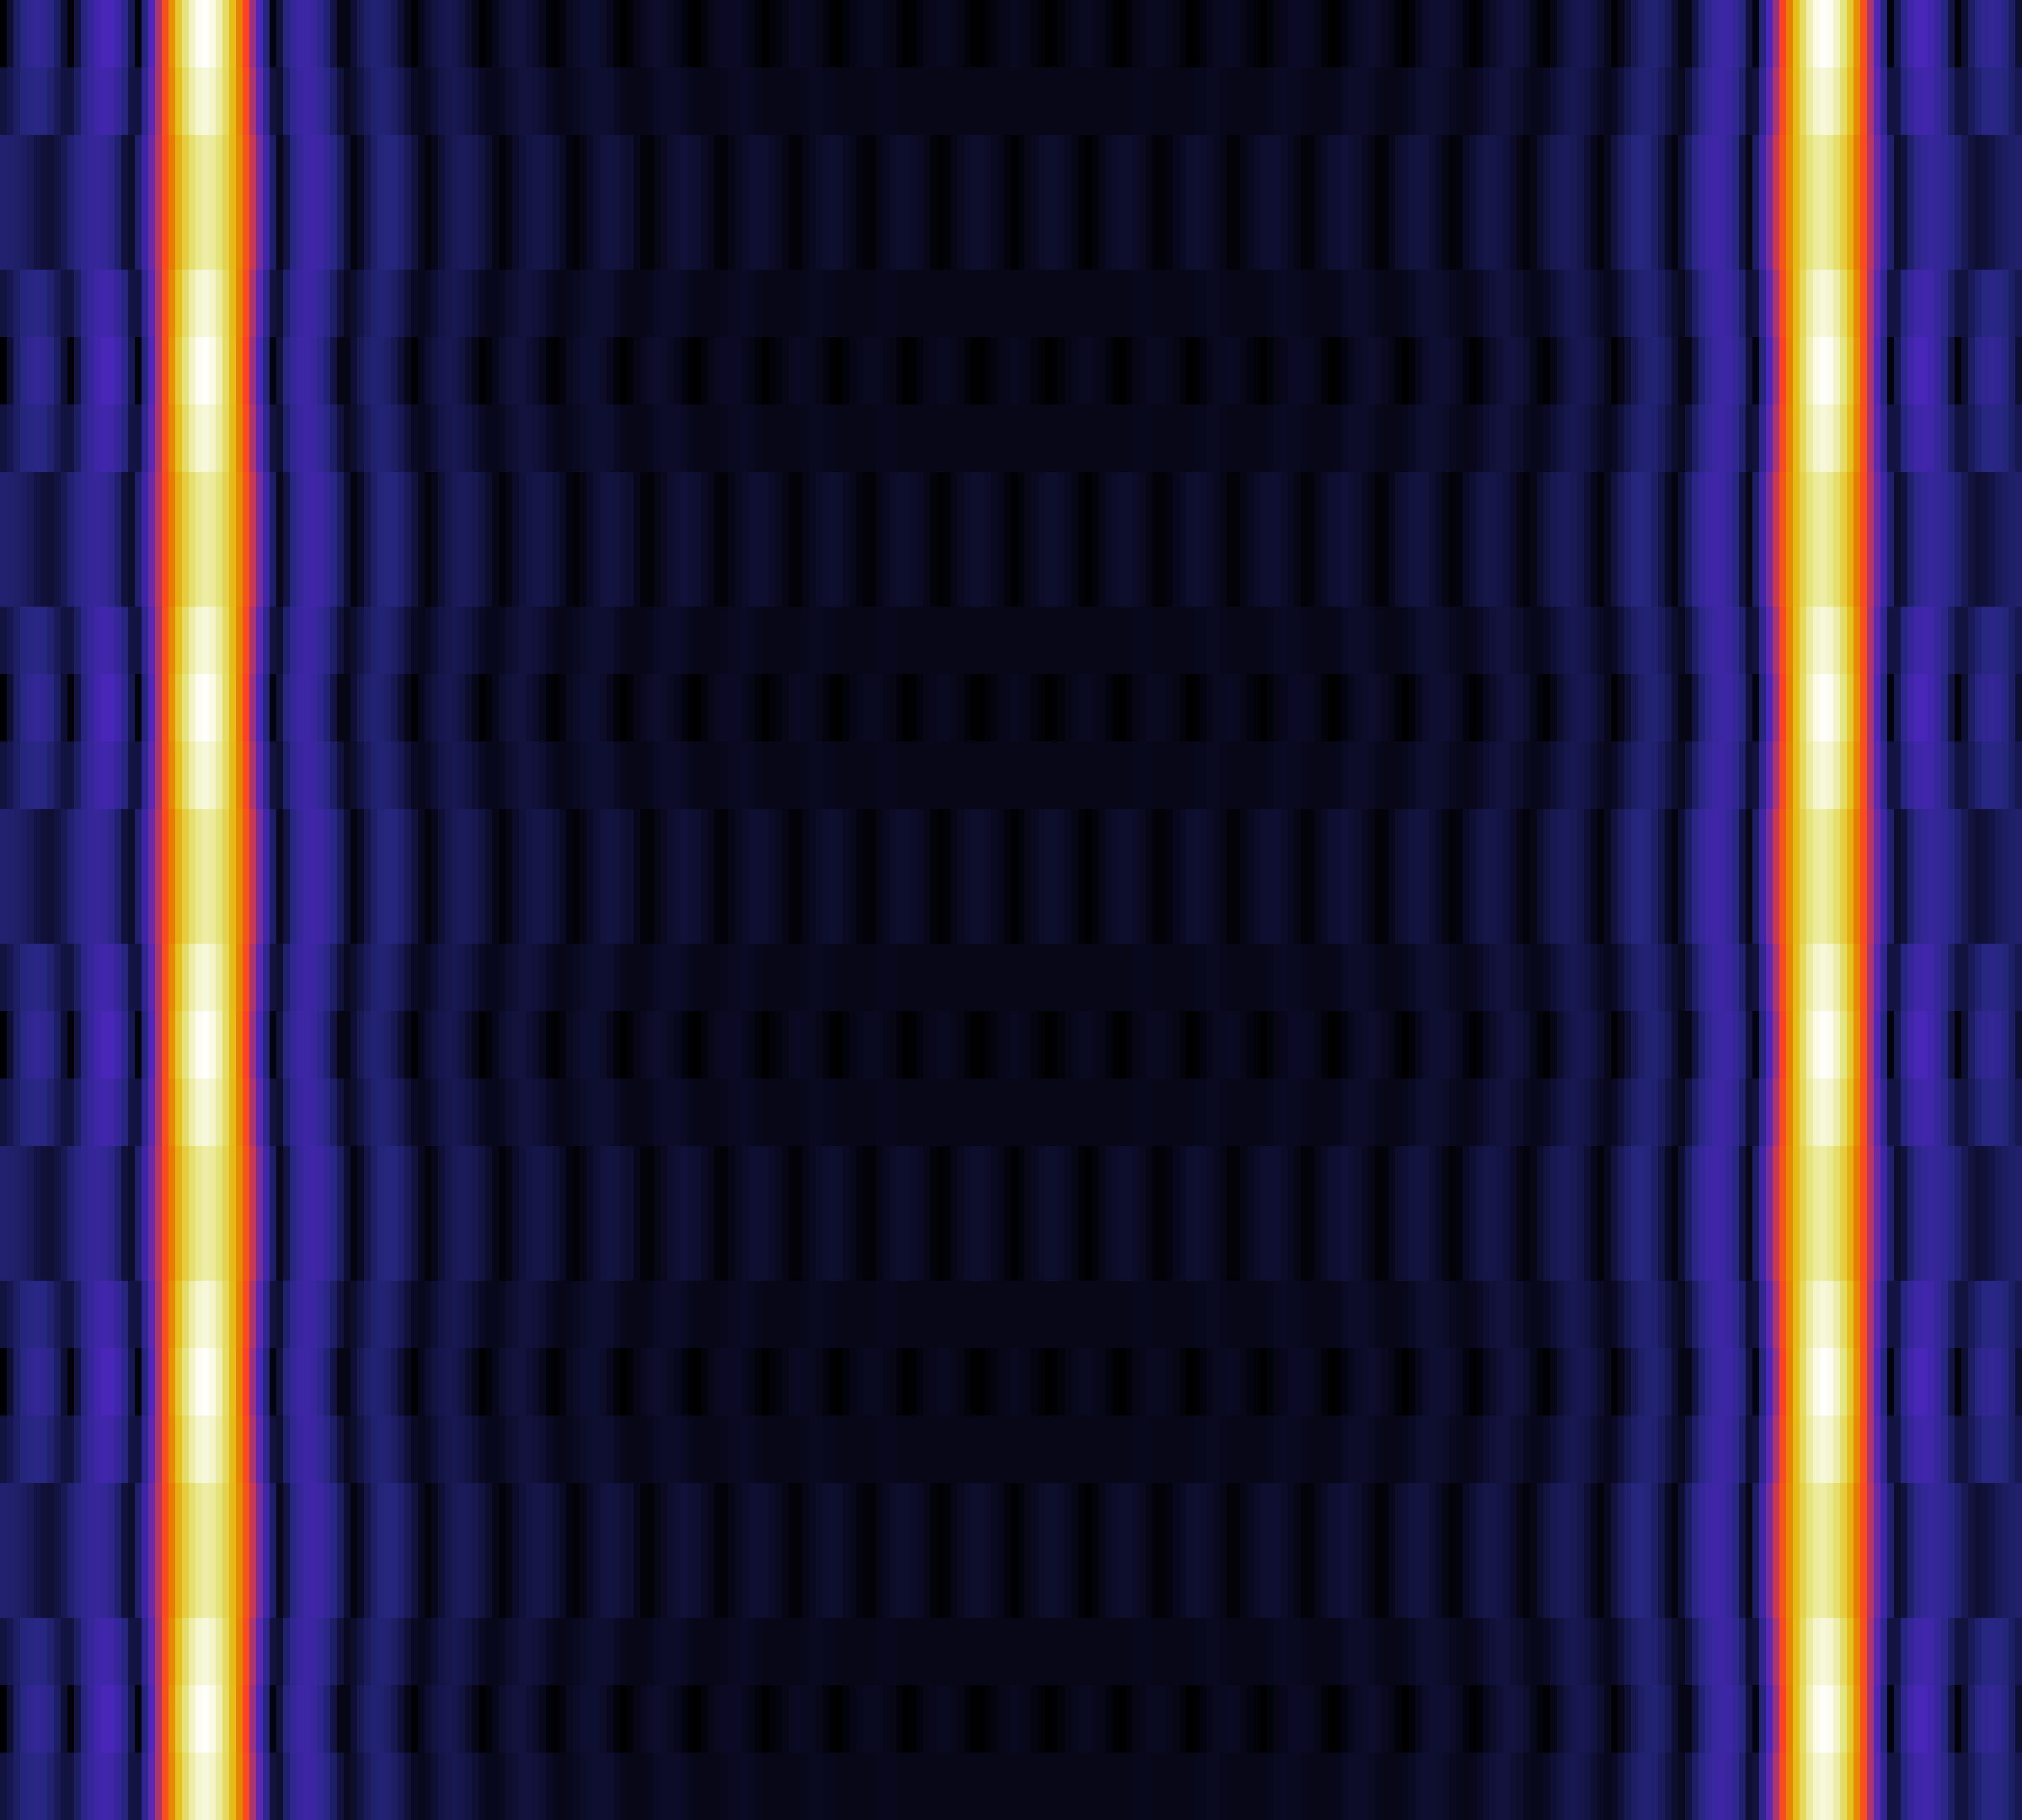
\includegraphics[width=0.5\textwidth]{./Imagenes/Espectrogramas/constante.jpg}
	            \caption{Representación gráfica de una señal de frecuencia constante}
	            \label{constante}
	        \end{figure}
	
	        \begin{figure}[h!]
	            \centering
	            
\includegraphics[width=0.5\textwidth]{./Imagenes/Espectrogramas/variable.jpg}
	            \caption{Representación gráfica de una señal con variación de frecuencia lineal $y_{[n]} = sen(\frac{2\pi}{17.75}n^2)$}
	            \label{variable}
	        \end{figure}
	De un análisis más profundo (el cual no se desarrolla) podemos determinar a su vez que la señal en estudio presenta un solapamiento de frecuencias mas altas que las capaces de recontruir a partir del muestreo dado.
	Este solapamiento se produce en los segmentos en los que las lineas de frecuencias predominantes “rebotan” contra los laterales de la matriz de espectro.
	
	Si bien siempre que se produzca un solapamiento se verá este “rebote”, la presencia del mismo no implica la existencia de solapamiento
	 ya que la señal puede llegar al máximo de frecuencia posible y luego comenzar a disminuir la frecuencia, lo cual produciría el mismo “rebote”
	  en la matriz pero no sería una señal con el mismo comportamiento.

\subsection{Determinación de la calidad de la discretización de $\omega$}
En una primer instancia se había elegido discretizar el dominio frecuencial en 30 valores equidistanciados entre $-\pi$ y $\pi$, debido a la periodicidad de la transformada de Fourier de tiempo discreto.
Para definir si nuestra primer discretización de $\omega$ nos provee de una aproximación suficientemente buena para analizar los espectrogramas decidimos aumentar en uno y dos órdenes de magnitud la primer discretización.

Estas diferentes discretizaciones se comparan en la figura \ref{comparacion} y lo que se puede observar a simple vista es que no existen comportamientos extraños en ninguna discretización, por lo que la primer
 elección de 30 valores ya nos brindaba una buena aproximación a lo que estaba sucediendo en la función original.

	         \begin{figure}[h!]
	            \centering
	            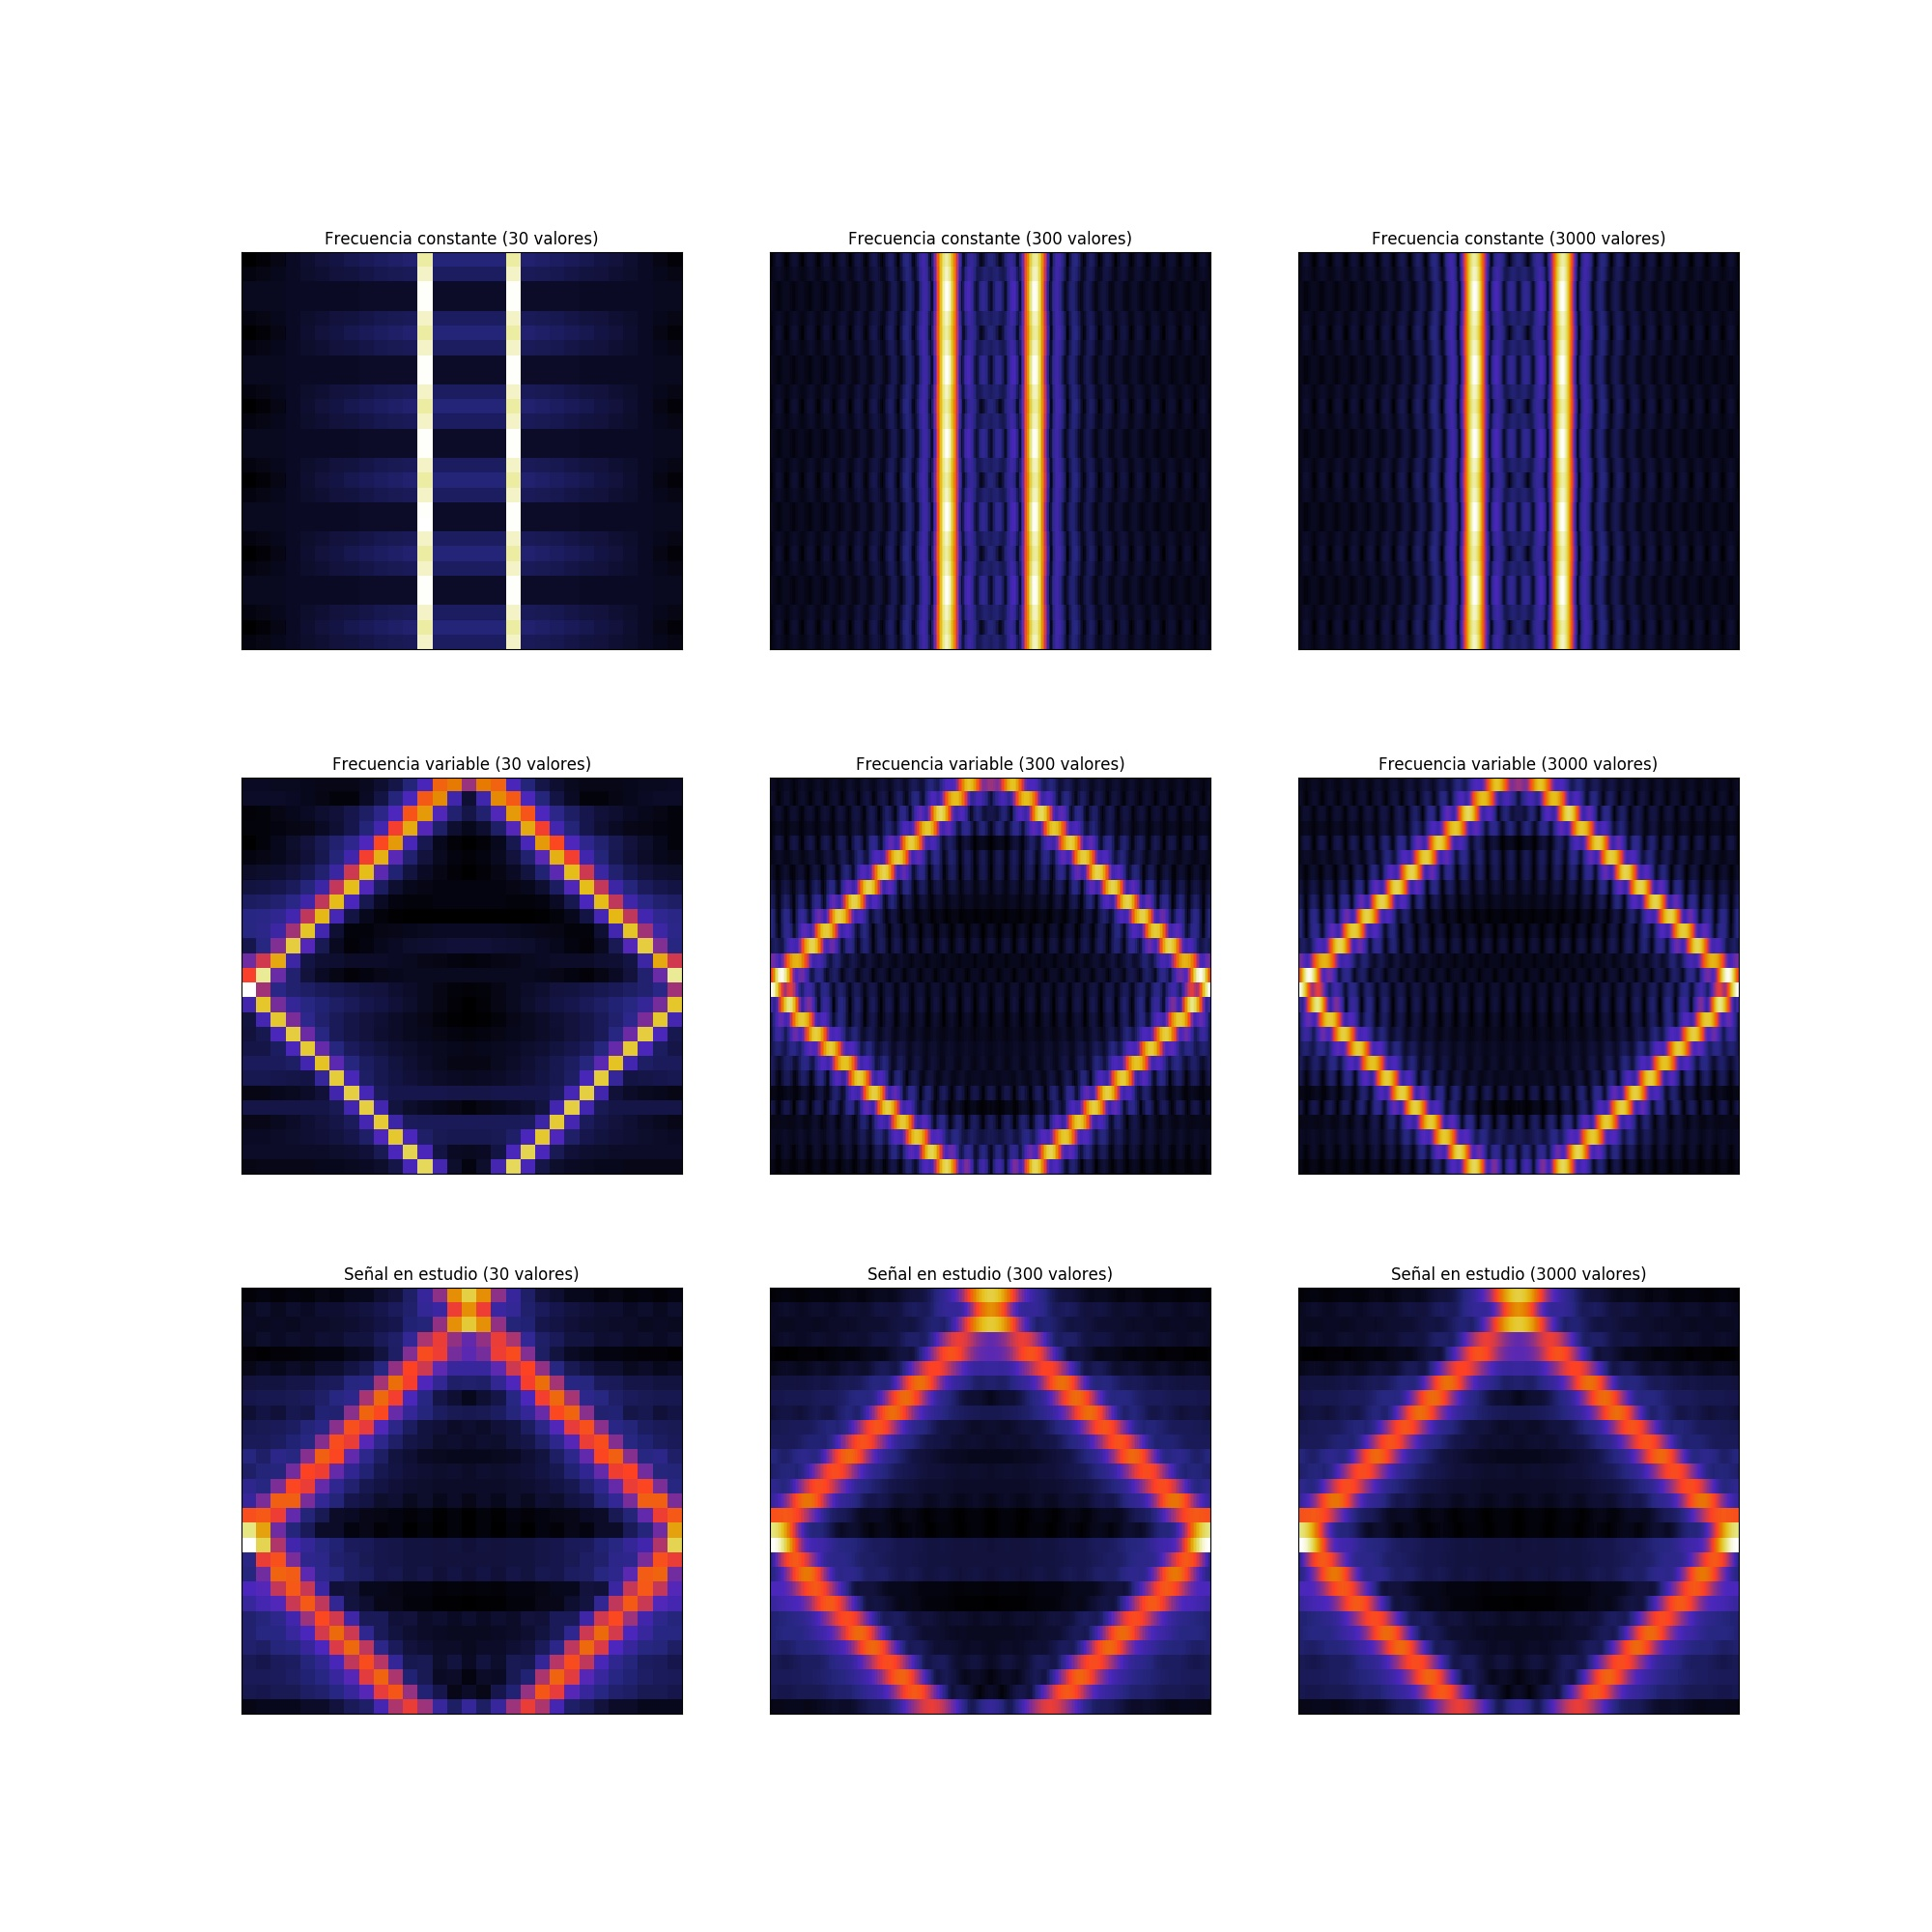
\includegraphics[width=\textwidth]{./Imagenes/Espectrogramas/merge.jpg}
	            \caption{Comparación de los espectrogramas  discretizando $\omega$ en 30, 300 y 3000 valores}
	            \label{comparacion}
	        \end{figure}
	    
De todas maneras se puede pensar que una discretización de 3000 valores no es lo suficientemente buena como para tener una idea de lo que sucede en la función estudiada, es por esto que se desarrolló la antitransformada
a partir de las discretizaciones de $\omega$, las cuales se comparan en el primer segmento de 30 muestras (ya que este es el largo de una muestra del espectrograma).
	         \begin{figure}[h!]
	            \centering
	            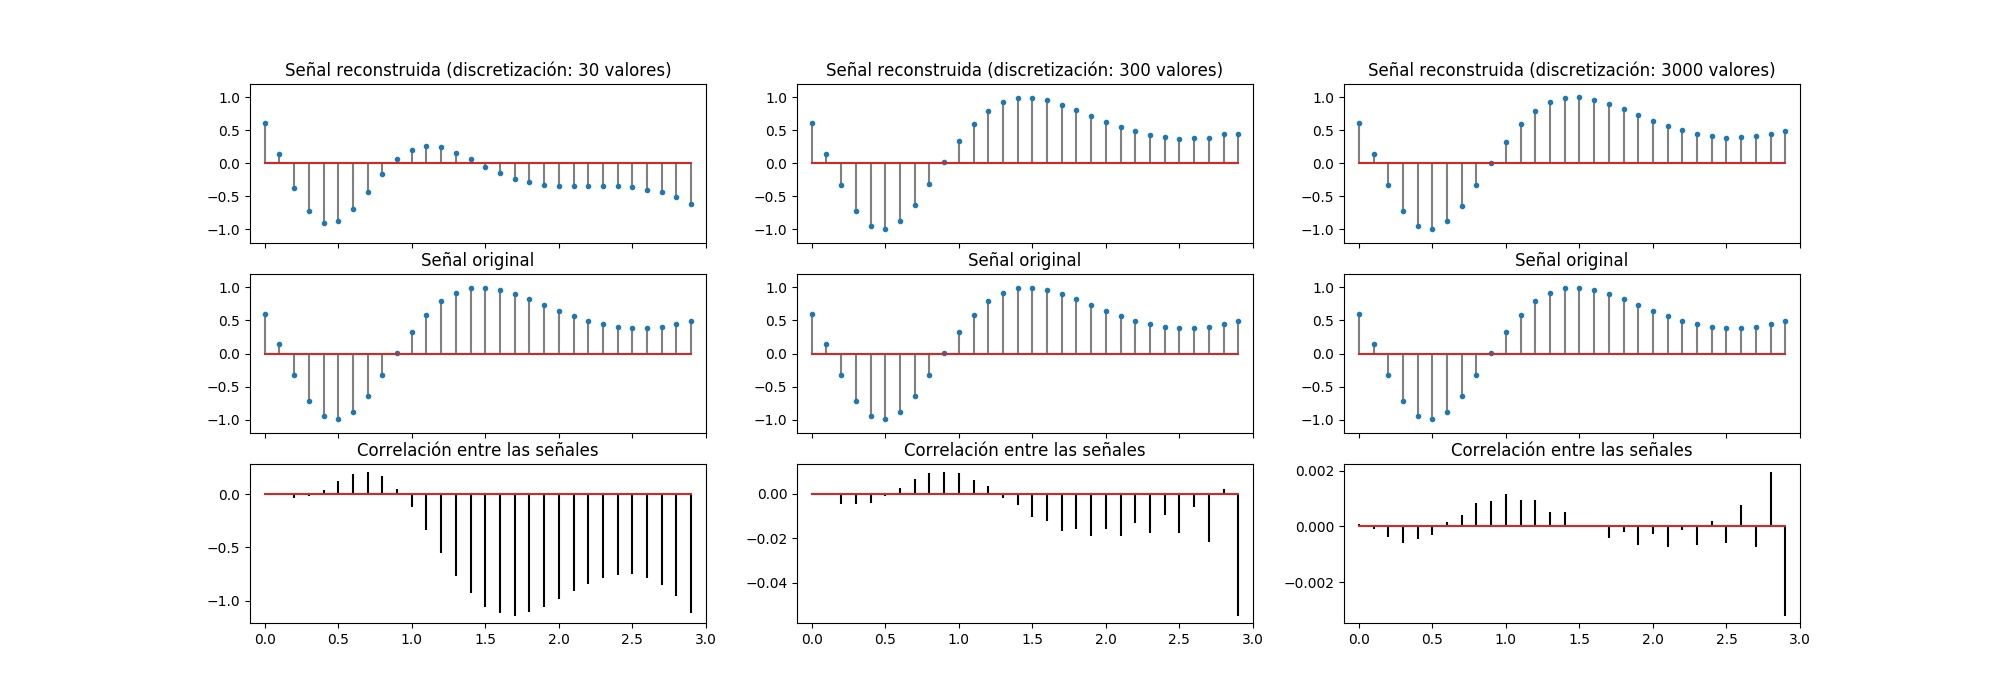
\includegraphics[width=\textwidth]{./Imagenes/antitransformada/comparacion.jpg}
	            \caption{Reconstrucción de la señal original a partir de las discretizaciones de $\omega$}
	            \label{recreacion}
	        \end{figure}
En la figura \ref{recreacion} se puede observar las comparaciones entre las señales recontruidas, si bien se observa que una discretización de $\omega$ en 30 valores no es suficiente para reconstruir la señal original,
a nuestro parecer es una discretización que provee una vaga idea de las frecuencias predominantes en la señal estudiada y es por esto que los espectrogramas de la figura \ref{comparacion} son muy similares.

La reconstrucción de la señal a partir de una discretización de $\omega$ en 3000 valores es una reconstrucción muy fiel a la señal original (con un error $<1\%$), por lo que se puede decir con bastante certeza que el espectrograma generado a partir de dicha discretización es representativo de la señal en estudio.
Así mismo, como observamos que los espectrogramas de 30 y 3000 valores de discretización son similares, podemos decir entonces que nuestra primer discretización (en 30 valores) era lo suficientemente buena para analizar la señal y compararla con otras señales.
	        
\newpage \section{Sistema masa-resorte-amortiguador discreto}

Como contrapartida de la ecuación diferencial que modela el comportamiento del sistema en estudio, se desarrolla la ecuación en diferencias contemplando las siguientes aproximaciones:

$$y'_{(t)} \approx \frac{y_{[n+1]}-y_{[n-1]}}{2T}$$

$$y''_{(t)} \approx \frac{y_{[n+1]} - 2 y_{[n]} + y_{[n-1]}}{T^2}$$

siendo $T$ el tiempo entre muestras. Si bien no es posible interpretar la derivada de una función discreta en el tiempo, las expresiones mostradas son una aproximación.


Por lo tanto, para aproximar la ecuación diferencial que simula al sistema del amortiguador, debemos reemplazar todas las apariciones de $y'$ e $y''$.

Siendo el sistema contínuo del amortiguador:

$$k_3 y''_{(t)} + k_2 y'_{(t)} + k_1 y_{(t)} = x_{(t)}$$

Nos queda que la ecuación en diferencia que aproxima al modelado continuo del sistema sería:

$$k_1 y_{[n]} + k_2 \left(\frac{y_{[n+1]}-y_{[n-1]}}{2T}\right) + k_3 \left(\frac{y_{[n+]1} - 2 y_{[n]} + y_{[n-1]}}{T^2}\right)= x_{[n]}$$

A partir de esta ecuación en diferencias se puede calcular la función de tranferencia del sistema, quedando la misma:

$$H_{(z)} = \frac{1}{\left(\frac{k_3}{T^2} - \frac{k_2}{2T}\right) z^{-1} + \left(k_1-\frac{2k_3}{T^2}\right) + \left(\frac{k_2}{2T} + \frac{k_3}{T^2}\right) z} $$


Reemplazando los valores de $k_1$, $k_2$, y $k_3$ por los correspondientes a la entrega anterior, y definiendo $T=0.1$ obtendríamos una discretización del sistema estudiado, obteniendo valores con una frecuencia de 10 Hz. De esta manera podemos reconstruir cualuier señal con un ancho de banda menor a 5 Hz, debido a que el amortiguador es un sistema mecánico suponemos que  no existirán variaciones de mayor frecuencia que esta.

$$ k_1 =1$$
$$k_2 =10$$
$$k_3=1$$

A partir de los valores elegidos la función de transferencia queda de la siguiente manera:

$$H_{(z)} = \frac{1}{50 z^{-1} - 190 + 150 z^{2}}$$

Utilizando el software xcos de scilab simulamos la respuesta del sistema utilizando transformada de laplace (sistema contínuo) para luego simular el sistema con la discretización definida y comparar los resultados.

        \begin{figure}[h!]
            \centering
            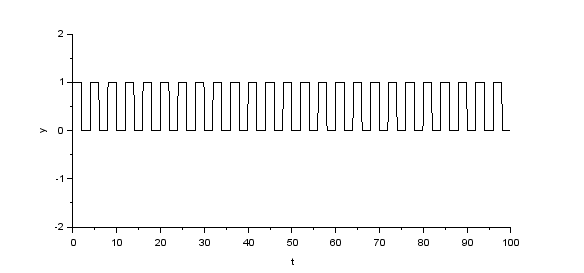
\includegraphics[width=0.7\textwidth]{./Imagenes/Simulaciones/entradaContinua.png}
            \caption{Entrada al sistema contínuo.}
            \label{entradaContinua}
        \end{figure}

        \begin{figure}[h!]
            \centering
            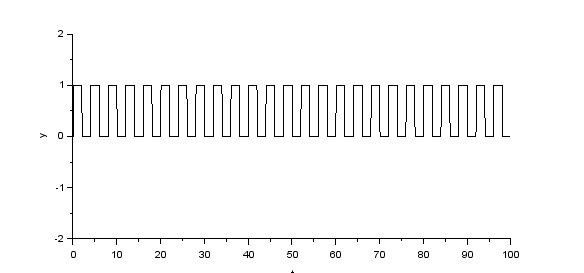
\includegraphics[width=0.7\textwidth]{./Imagenes/Simulaciones/entradaDiscreta.png}
            \caption{Entrada al sistema discreto.}
            \label{entradaDiscreta}
        \end{figure}
        
         \begin{figure}[h!]
            \centering
            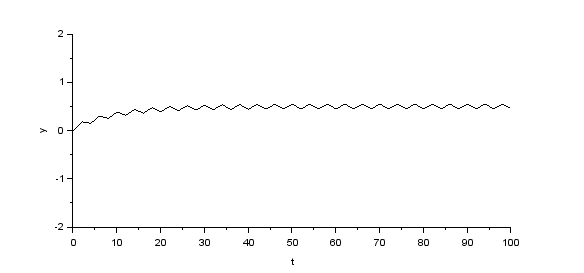
\includegraphics[width=0.7\textwidth]{./Imagenes/Simulaciones/salidaContinua.png}
            \caption{Salida resultante de simular el sistema con un sistema LTI contínuo.}
            \label{salidaContinua}
        \end{figure}
        
              \begin{figure}[h!]
            \centering
            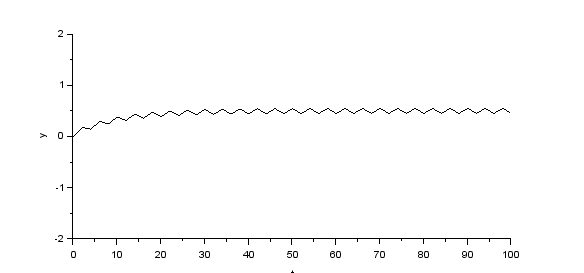
\includegraphics[width=0.7\textwidth]{./Imagenes/Simulaciones/salidaDiscreta.png}
            \caption{Salida resultante de simular el sistema con un sistema LTI discreto.}
            \label{salidaDiscreta}
        \end{figure}


Como se puede observar de las gráficas obtenidas, la discretización del sistema con un intervalo de muestreo de $0,1$ segundos resulta en una muy buena discretización para el sistema en estudio.
No observandose una diferencia entre las salidas de los sistemas contínuo y discreto.







    
\end{document}

